My years of experience dealing with high DOF robots was the catalyst for my thesis, the DARPA Robotics Challenge (DRC) was the fuel that kept my Hubo-Ach controller development thriving.
Having an event that required multi-disciplinary collaboration in a short development time frame was the perfect place for me to test the viability of my controller.\\

\noindent \textbf{Overview of the DARPA Robotics Challenge:} In July 2012 DARPA released a solicitation for proposals to compete in the DARPA Robotics Challenge.
The DRC is a challenge that is in direct response to the Tsuanmi in Fukushima in 2011 (check this).
The challenge is to have a robot be able to use human tools, human vehicles and preform human tasks in an un-structured un modified human environment.
We applied for the grant.
Fig.~\ref{fig:drcEvents} depict Hubo2+ (KHR-4) preforming the eight given tasks.  
The photographs are meant to help you \textit{imagine} that the robot is capable of preforming these tasks not to state that the robot has already completed these tasks at the time of application.  
The events are:
\begin{itemize}
\item \textbf{Event 1:} Driving an un-modified human vehicle
\item \textbf{Event 2:} Walking over rough, un-even terrain
\item \textbf{Event 3:} Removing debris from regions of interest
\item \textbf{Event 4:} Opening and navigating through multiple doors and hallways
\item \textbf{Event 5:} Climb an industrial ladder
\item \textbf{Event 6:} Break through a wall using un-modified human tools
\item \textbf{Event 7:} Turn a valve
\item \textbf{Event 8:} Replace a pump (note: this was replaced by a hose insertion task)
\end{itemize}

In October 2012 we received word that we are a Track-A team for the DRC.
This means that we are competing against NASA, Raythion, CMU and a team from Japan.
One of the keys to our team is our collaboration.
We are partnered with WPI, Georgia Tech, University of Delaware, Swarthmore, Purdue, Ohio State (check that) and RAINBOW (a company that rose from the Hubo Lab at Korea Advanced Institute of Science and Technology (KAIST)).
Each partner would be responsible with one event.
We will then combine our efforts into one master controller that is capable of doing all the given tasks.
Having a multi-process system that also gives us the ability for our partners to share their controllers without having to integrate their code.  
Controllers run independently.

\begin{figure}[thpb]
  \centering
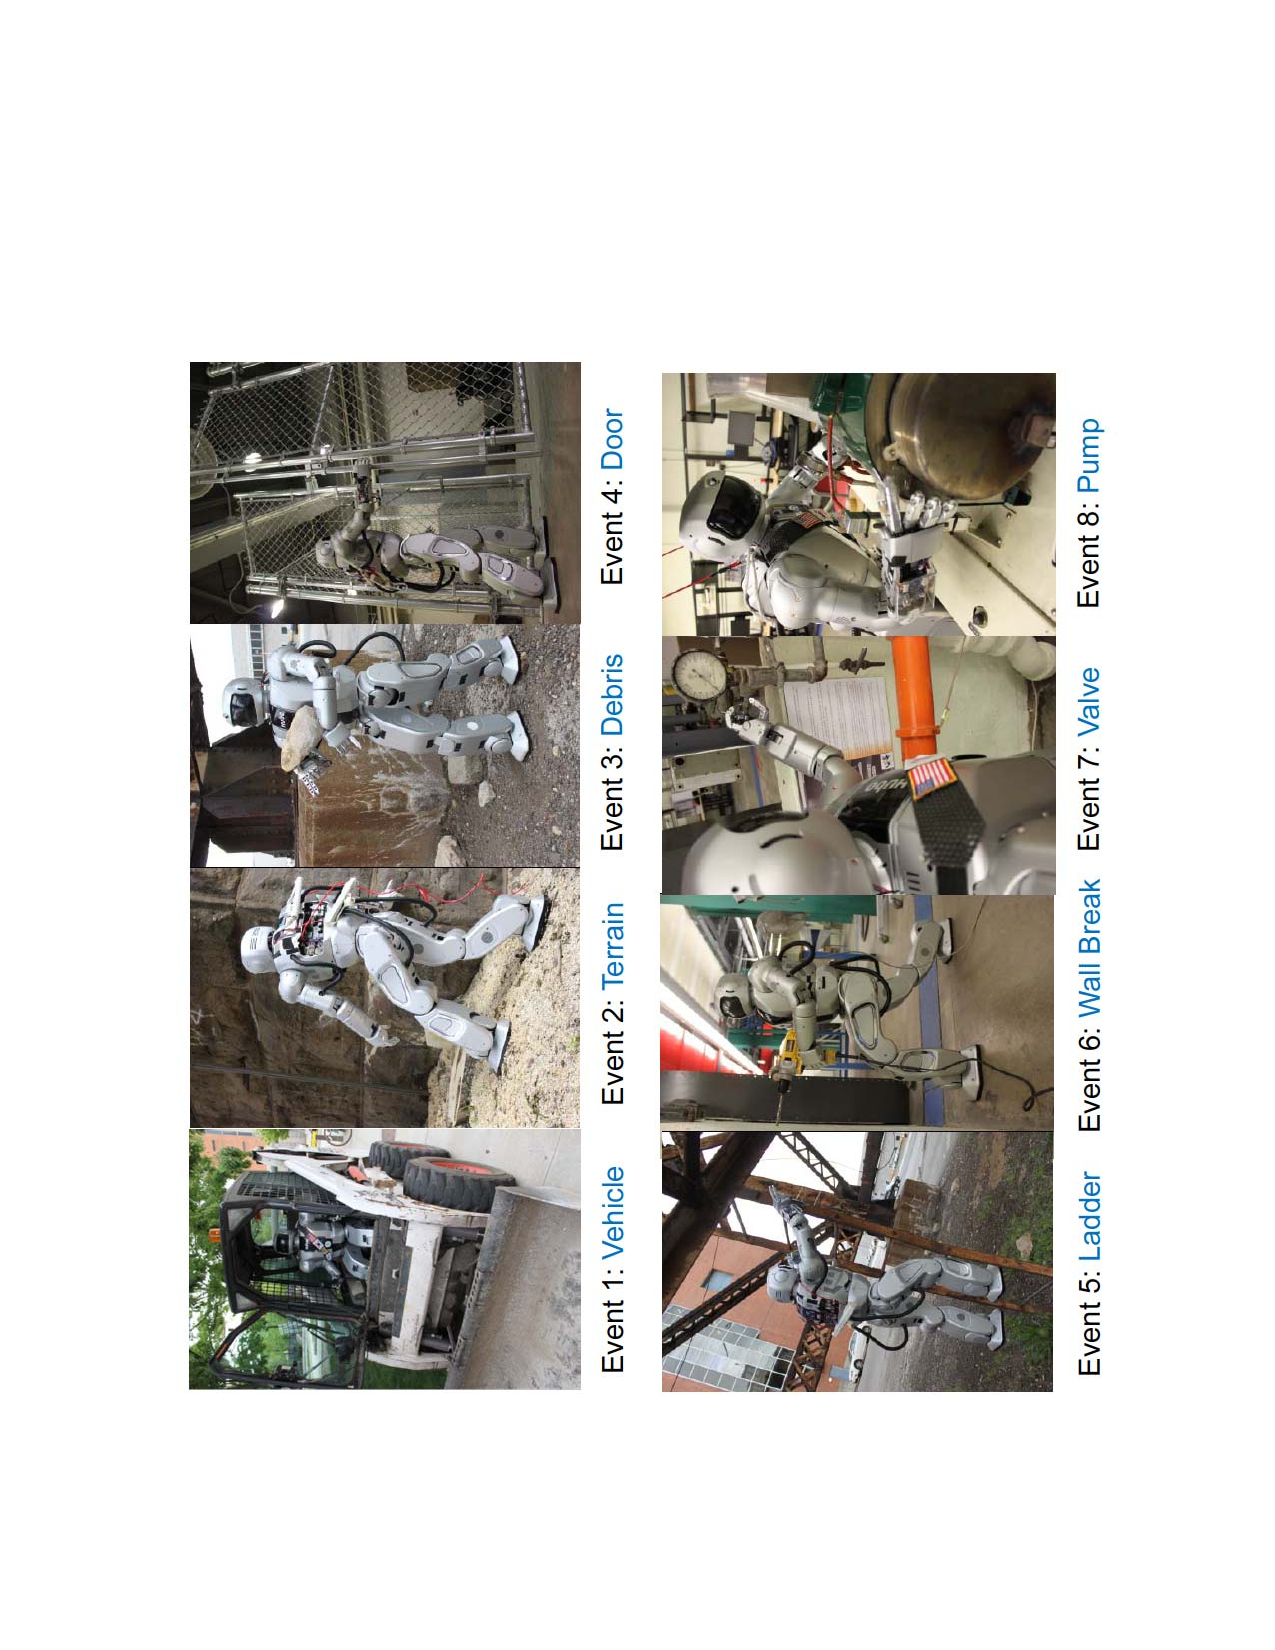
\includegraphics[height=1.0\columnwidth, angle=-90]{./background/pix/drcEvents.pdf}
  \caption{DARPA Robot Challenge Events.  Pictures depict the Hubo2+ (KHR-4) preforming the eight given tasks.  The photographs are meant to help you \textit{imagine} that the robot is capable of preforming these tasks.  The events are - Event 1: Driving an un-modified human vehicle; Event 2: Walking over rough, un-even terrain; Event 3: Removing debris from regions of interest; Event 4: Opening and navigating through multiple doors and hallways; Event 5: Climb an industrial ladder; Event 6: Break through a wall using un-modified human tools; Event 7: Turn a valve; Event 8: Replace a pump (note: this was replaced by a hose insertion task).  All photographs were staged and taken by Daniel M. Lofaro.  Picture montage taken from Dr. Paul Oh's meeting to DARPA at the DRC Kickoff meeting, October 23-25, 2012.\cite{drOhDARPA}    }
  \label{fig:drcEvents}
\end{figure}

